% Figure: matched motion-signal controls. Rendered by render_tables.py via render_figures.motion_forest from the
% motion-controls analysis outputs; nothing numeric is typed here.
% supplement-ref tab:s-motion-scramble=S28
% supplement-ref tab:s-motion-purity=S29
\begin{figure}[!htbp]
\centering
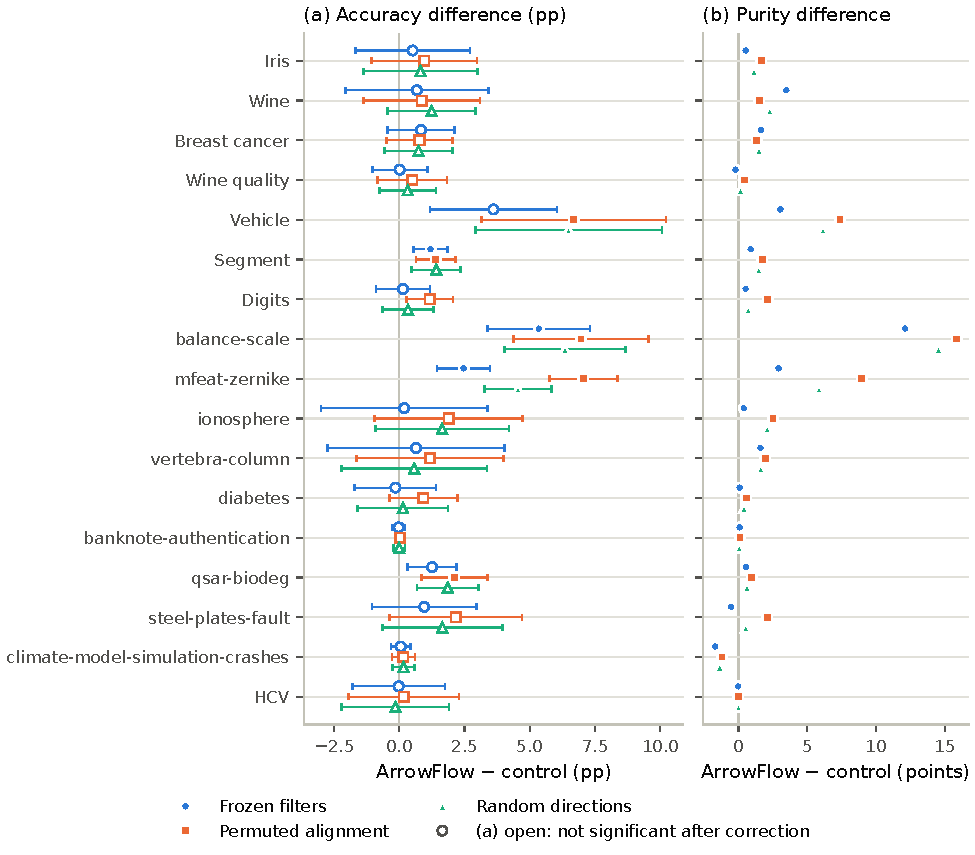
\includegraphics[width=0.92\textwidth]{figures/data/fig8_motion_forest.pdf}
\caption{\textbf{Is it the signal that helps?} (a)~ArrowFlow's accuracy minus that of each control, in percentage points, with 95\% intervals (not simultaneous); positive favors ArrowFlow. Frozen filters: the hidden filters never move. Permuted alignment: each motion reaches a filter of the same layer drawn at random, afresh in every batch. Random directions: the directions of the motions are shuffled. Both scrambled controls keep the number of motions, their sizes and their total weight. Filled marks in panel (a) remain significant after a Holm correction across the seventeen datasets within each control: 3 datasets for frozen filters, 5 for permuted alignment and 3 for random directions. The intervals are not adjusted for multiple comparisons, so an open mark's interval can exclude zero. In panel (a), ArrowFlow is more accurate than frozen filters on 14 of the 17 datasets, than permuted alignment on 17 and than random directions on 16. (b)~Neighborhood purity, how often an example's nearest training examples share its class: ArrowFlow minus each control, in percentage points, on the test rows; descriptive, with no interval and no test, so its marks carry no fill coding. ArrowFlow is purer than all three controls on 13 of the 17 datasets. In both panels, a scramble's mark to the right of the mark of frozen filters means that the scramble is less accurate than frozen filters, or in panel~(b) less pure. Tables~S28 and~S29 give these comparisons directly. HCV: hepatitis C virus.}
\label{fig:motion-forest}
\end{figure}
